

% -------------------- DOCUMENT --------------------
\begin{document}
\maketitle

% -------------------- ABSTRACT --------------------
\begin{abstract}
The rising global burden of ocular diseases demands early, reliable, and interpretable diagnostic solutions. Traditional diagnosis depends heavily on expert ophthalmologists, limiting large-scale screening. This project proposes an Explainable AI-based multiclass ocular disease detection system using deep learning and interpretability techniques. Our approach employs CNNs for feature extraction and classification of diabetic retinopathy, glaucoma, cataract, and macular degeneration. Grad-CAM integration highlights pathological regions influencing predictions. The system provides an intuitive interface where clinicians upload retinal images and receive predictions with explanations, enabling trust in the diagnostic process. This work reduces diagnostic workload, improves screening accuracy, and ensures interpretable AI assistance. The novelty lies in combining high-performance classification with visual explainability for practical, reliable healthcare applications.
\end{abstract}

% -------------------- KEYWORDS --------------------
\begin{IEEEkeywords}
Explainable AI, Deep Learning, CNN, Grad-CAM, Ocular Disease Detection, Computer Vision, Medical Imaging, Multi-class Classification
\end{IEEEkeywords}

% -------------------- INTRODUCTION --------------------
\section{Introduction}

Ocular diseases affect millions worldwide and are leading causes of preventable blindness. Diabetic retinopathy, glaucoma, cataracts, and age-related macular degeneration often progress silently until irreversible damage occurs~\cite{R1}. Vision impairment prevalence is substantially higher in low- and middle-income regions with limited ophthalmologic care~\cite{R2}. This underscores the need for accessible, accurate, and timely diagnostic solutions supporting early intervention.

Traditional diagnosis relies on manual examination of retinal fundus images by experienced ophthalmologists. While clinically standard, these methods are time-consuming, labor-intensive, and subject to inter-observer variability, subjective interpretation, and specialist scarcity~\cite{R3,R4}. As ocular disease burden rises, automated intelligent screening systems are urgently needed to augment clinical decision-making.

Deep learning and computer vision advances have revolutionized medical image analysis. CNNs demonstrate remarkable capabilities in learning discriminative features from medical images, achieving performance comparable to or exceeding human experts~\cite{R1,R5}. These models automatically extract hierarchical representations, capturing subtle patterns difficult for humans to detect consistently. Transfer learning from large-scale datasets like ImageNet enables effective training with limited medical imaging data~\cite{R6,R7}.

Despite technological progress, lack of model interpretability remains a critical barrier to clinical adoption. Deep neural networks are "black boxes" providing predictions without transparent reasoning~\cite{R3,R4}. In high-stakes medical applications, clinicians require not only accurate predictions but also understandable explanations supporting informed decisions. Absence of interpretability limits clinical trust, hinders error analysis, and prevents meaningful AI integration into healthcare workflows~\cite{R8,R9}.

Explainable Artificial Intelligence (XAI) addresses interpretability challenges by making model decisions transparent and comprehensible. Methods like Gradient-weighted Class Activation Mapping (Grad-CAM) and Local Interpretable Model-agnostic Explanations (LIME) generate saliency maps highlighting regions of interest, enabling clinicians to understand which features influenced diagnostic conclusions~\cite{R3,R4}.

This research develops an Explainable AI-based multiclass ocular disease detection system addressing both high accuracy and transparency. The proposed framework integrates state-of-the-art CNN architectures with explainability techniques to classify multiple diseases from retinal fundus images. Grad-CAM visualization provides interpretable heatmaps localizing pathological regions, enhancing clinical trust and facilitating prediction validation.

The paper organization: Section~\ref{sec:theoretical} provides theoretical background. Section~\ref{sec:related} presents comprehensive literature review. Section~\ref{sec:methodology} describes the proposed methodology. Section~\ref{sec:results} presents experimental results. Section~\ref{sec:hybrid} discusses hybrid approaches. Section~\ref{sec:issues} identifies challenges. Section~\ref{sec:future} outlines future directions. Section~\ref{sec:conclusion} concludes.

% -------------------- THEORETICAL BACKGROUND --------------------
\section{Theoretical Background}
\label{sec:theoretical}

This section establishes foundational concepts for explainable AI-based ocular disease detection: retinal anatomy, imaging modalities, deep learning architectures, and explainability paradigms.

\subsection{Retinal Anatomy and Ocular Pathologies}

The retina is multi-layered neural tissue converting light into neural signals. The macula contains the fovea for high-acuity central vision; the optic disc marks retinal nerve fiber convergence; retinal vasculature provides metabolic support.

Ocular diseases manifest through characteristic structural changes. Diabetic retinopathy, the leading working-age blindness cause, results from chronic hyperglycemia damaging retinal microvasculature, showing microaneurysms, hemorrhages, and exudates in early stages; advanced stages feature neovascularization and fibrous tissue. Glaucoma involves progressive optic nerve damage from elevated intraocular pressure, revealing optic disc cupping and rim thinning. Age-related macular degeneration (AMD) affects central vision: dry AMD presents drusen deposits and pigment epithelium changes; wet AMD involves choroidal neovascularization with fluid and hemorrhage. Cataracts affect lens clarity, impacting fundus image quality.

\subsection{Retinal Imaging Modalities}

Fundus photography is the primary non-invasive retinal imaging modality. Color fundus cameras capture wide-field posterior retina images using visible light, covering 30-50 degrees retinal field. Digital cameras generate high-resolution images (typically 2048×1536+ pixels) preserving anatomical details. Flash illumination minimizes discomfort while ensuring adequate exposure; automated alignment assists non-specialist operators; standardized calibration ensures consistency.

Optical Coherence Tomography (OCT) provides cross-sectional retinal layer imaging with micrometer resolution. While OCT excels at structural changes, fundus photography remains primary for screening due to lower cost, simpler operation, and established protocols. Fluorescein angiography visualizes vascular dynamics but requires intravenous dye, limiting routine screening.

\subsection{Convolutional Neural Networks for Medical Imaging}

CNNs form the foundation of modern medical image analysis, processing grid-structured data exploiting spatial locality and translation invariance through parameter sharing. Hierarchical architectures extract increasingly abstract features.

Convolutional layers apply learnable filters detecting local patterns (edges, textures, shapes); multiple parallel filters enable diverse detection. Pooling layers reduce spatial dimensionality through aggregation, providing translation invariance. Activation functions (ReLU and variants) introduce nonlinearity addressing gradient vanishing. Batch normalization standardizes layer inputs, accelerating convergence; dropout regularization prevents overfitting.

Transfer learning leverages pre-trained models from large-scale datasets like ImageNet. Lower layers learn generic features; higher layers capture task-specific concepts. Fine-tuning adjusts pre-trained weights using domain-specific medical images, requiring substantially less data than random initialization—particularly effective for limited medical imaging datasets.

\subsection{Explainability in Deep Learning}

Explainability techniques address deep neural network "black box" nature through three paradigms: ante-hoc interpretability (transparent architectures), post-hoc explanation generation (opaque models), and example-based explanation (case retrieval).

Gradient-based methods compute input attributions by backpropagating prediction scores to input pixels. Simple gradients highlight high-magnitude pixels indicating perturbation sensitivity; Integrated Gradients accumulate gradients along baseline-to-input paths satisfying sensitivity and implementation invariance; SmoothGrad reduces noise through Gaussian-perturbed averaging.

Class Activation Mapping (CAM) generates coarse localization maps indicating discriminative regions by computing weighted sums of final convolutional feature maps. Grad-CAM generalizes CAM to arbitrary architectures using gradients for feature importance weighting, enabling visualization without architectural constraints.

Attention mechanisms provide intrinsic interpretability by computing importance weights over spatial locations. Self-attention learns context-dependent scoring, directing focus toward relevant regions. However, attention weights represent intermediate computations, not complete explanations.

Perturbation methods like LIME approximate local model behavior using interpretable surrogates, perturbing inputs by masking regions and training linear classifiers predicting outputs. Linear model coefficients indicate regional importance. While model-agnostic, perturbation methods require numerous forward passes, increasing computational cost.

\subsection{Performance Evaluation Metrics}

Medical diagnostic systems use metrics balancing sensitivity to true positives against specificity to true negatives. Accuracy measures overall correctness but misleads for imbalanced datasets.

Precision quantifies positive prediction correctness, critical when false positives incur significant costs. Recall/sensitivity measures identified actual positive case fraction, crucial for minimizing missed diseases. F1-score computes precision-recall harmonic mean, providing balanced performance.

For multi-class problems, metrics are computed per-class and aggregated via macro-averaging (unweighted class mean) or micro-averaging (aggregating counts before computing). Area Under ROC Curve (AUC-ROC) provides threshold-independent performance, plotting true positive against false positive rate.

Confusion matrices enable detailed error analysis by tabulating predicted versus actual assignments, revealing failure modes like systematic confusion between similar pathologies. Certain error types carry different clinical consequences—false negatives for sight-threatening conditions are more serious than false positives requiring confirmatory testing.

% -------------------- RELATED WORK --------------------
\section{Related Work}
\label{sec:related}

This section reviews deep learning techniques for automated ocular disease detection, organized by methodology with implementation details, datasets, and contributions.

\subsection{Deep Learning Architectures for Disease Classification}

Deep learning evolved from single-disease binary classifiers to sophisticated multi-class systems detecting multiple pathologies.

Raj et al.~\cite{R1} employed transfer learning with VGG-16, ResNet-50, and InceptionV3 initialized from ImageNet weights with custom classification heads. Data augmentation addressed dataset limitations and class imbalance. Evaluation on Messidor and DRIVE datasets achieved 89\% accuracy. However, lack of explainability mechanisms limited clinical deployment feasibility.

Li et al.~\cite{R2} surveyed machine learning for ocular disease detection across modalities. The review analyzed preprocessing (CLAHE, morphological operations, color transformations), feature extraction (SIFT/HOG to CNN representations), and classification (SVMs, Random Forests, CNNs). Key challenges included limited annotated datasets, class imbalance, and cross-equipment generalization. While CNNs achieved promising accuracy, most operated as black boxes, limiting clinical trust.

Hemal and Saha~\cite{R10} introduced an explainable meta-classifier combining MobileNetV2, InceptionV3, DenseNet121, and EfficientNetB4. ImageNet pre-trained models were fine-tuned on retinal datasets; ensemble meta-classifier used weighted voting. Evaluation on ODIR-5K (5,000 patients, 8 labels) and RFMiD (3,200 images, 29 conditions) achieved 98.1\% accuracy, 98.2\% precision, 98.1\% sensitivity. Grad-CAM generated attention maps highlighting disease-influencing regions corresponding to known pathological features. This demonstrated high-accuracy multi-label classification with interpretability, though ensemble complexity limited resource-constrained deployment.

Hasan et al.~\cite{R6} developed DIA-VXNET using transfer learning with feature fusion. Preprocessing used CLAHE (clip 2.0, tile 8×8) and unsharp masking with adaptive Gaussian filtering. Hybrid architecture integrated ResNet-50, InceptionV3, and DenseNet-169 features via transition blocks with concatenation, batch normalization, and 1×1 convolutions. Evaluation on Messidor-2, IDRiD, and APTOS 2019 achieved 96.8\% accuracy with AUC exceeding 0.98 for diabetic retinopathy, diabetic macular edema, cataracts, and normal conditions. Multi-scale fusion captured global patterns and local details, though focus remained on diabetic eye diseases.

Vidivelli et al.~\cite{R5} optimized deep learning models through hyperparameter tuning and architecture search. The study compared AlexNet, VGG, ResNet, and EfficientNet, exploring learning rates (constant, step decay, exponential, cosine annealing), batch sizes (16-128), optimizers (SGD, Adam, RMSprop, AdamW), and regularization strategies. Grid and random search on 15,000 proprietary fundus images across 5 categories yielded 3-8\% accuracy improvements. EfficientNet-B4 with cosine annealing, AdamW, and moderate augmentation achieved 95.3\% best performance, emphasizing methodical model selection importance.

\subsection{Explainability Techniques in Medical Imaging}

Explainability became critical for clinical AI deployment, making predictions interpretable to medical professionals.

Agarwal and Mitra~\cite{R3} reviewed explainable AI for medical imaging, categorizing methods into post-hoc (gradient-based: vanilla gradients, Integrated Gradients, SmoothGrad; CAM-based: CAM, Grad-CAM, Grad-CAM++, Score-CAM; perturbation: LIME, SHAP) and intrinsic interpretability (attention mechanisms, prototype learning, concept-based models). Evaluation across fidelity, interpretability, computational efficiency, and architectural applicability showed Grad-CAM as most adopted due to model-agnostic nature, efficiency, and intuitive visual explanations. Recommendations emphasized user studies validating explanation utility and standardized evaluation frameworks.

Selvaraju et al.~\cite{R8} introduced Grad-CAM for visual explanations via gradient-based localization. The method computes importance weights for final convolutional feature maps by global average pooling gradients: $\alpha_k^c = \frac{1}{Z}\sum_i\sum_j \frac{\partial y^c}{\partial A_{ij}^k}$, where $y^c$ is pre-softmax class score and $A^k$ is the $k$-th feature map. Final localization: $L_{Grad-CAM}^c = ReLU(\sum_k \alpha_k^c A^k)$. Unlike CAM requiring specific architectures, Grad-CAM applies to arbitrary CNNs. Validation on ImageNet, image captioning, and visual question answering showed consistent class-discriminative localization. Human studies demonstrated Grad-CAM helps establish appropriate trust, identifying failure modes and model strength discrimination. For medical imaging, Grad-CAM enables clinicians to verify predictions based on relevant anatomical features versus spurious correlations.

Islam et al.~\cite{R4} integrated multiple interpretability techniques for complementary perspectives, combining Grad-CAM, Integrated Gradients, LIME, SHAP, and attention visualization. Evaluation on ChestX-ray14, Messidor, and Camelyon16 for pneumonia, diabetic retinopathy, and cancer detection showed multi-faceted explainability offers more comprehensive insights. Grad-CAM excelled at coarse localization; Integrated Gradients provided finer attribution; LIME communicated effectively through superpixels. User studies with radiologists and ophthalmologists showed multi-method explanations increased confidence and facilitated error detection, though computational overhead limited real-time deployment.

\subsection{Generative Models and Data Augmentation}

Synthetic data generation addresses data scarcity and class imbalance in medical imaging.

Waisberg et al.~\cite{R9} surveyed generative AI in ophthalmology, examining GANs (adversarially trained generator-discriminator networks), VAEs (probabilistic latent representations), and Diffusion Models (iterative denoising). GANs generated realistic fundus images of diabetic retinopathy lesions, glaucomatous discs, and AMD changes. Style transfer enabled cross-device adaptation; synthetic oversampling addressed class imbalance; privacy-preserving data enabled training without exposing patient information. Applications included automated report generation and image quality enhancement. However, generated images require clinical realism validation and absence of misleading features. Synthetic data introduction needs careful evaluation ensuring models learn genuine patterns versus artifacts. Regulatory considerations remain unclear; rigorous validation comparing synthetic versus real data training is needed before clinical deployment.

% -------------------- PROPOSED METHODOLOGY --------------------
\section{Proposed Methodology}
\label{sec:methodology}

Our proposed explainable AI framework integrates deep learning-based classification with Grad-CAM visualization to provide transparent and interpretable ocular disease diagnosis. The system architecture comprises preprocessing, feature extraction, classification, and explanation generation modules.

\subsection{Data Preprocessing and Augmentation}

Fundus images undergo standardized preprocessing including resizing to 224×224 pixels, normalization using ImageNet statistics, and contrast enhancement via CLAHE. Data augmentation techniques including rotation (±15°), horizontal flipping, brightness adjustment (±20\%), and Gaussian noise addition address limited dataset size and improve model robustness.

\subsection{CNN Architecture and Transfer Learning}

We employ transfer learning with pre-trained CNN architectures (ResNet-50, InceptionV3, EfficientNet-B4) initialized from ImageNet weights. Final classification layers are replaced with custom fully connected layers for multi-class disease classification. The model is fine-tuned end-to-end using categorical cross-entropy loss and Adam optimizer with learning rate scheduling.

\subsection{Grad-CAM Visualization for Explainability}

Grad-CAM generates visual explanations highlighting pathologically relevant regions influencing predictions. For each predicted class, gradients of the class score are backpropagated to the final convolutional layer to compute feature map importance weights. The weighted combination of feature maps produces a coarse localization map indicating discriminative regions, which is upsampled and overlaid on the original image as a heatmap.

% -------------------- RESULTS AND VISUALIZATION --------------------
\section{Experimental Results}
\label{sec:results}

This section presents the experimental results demonstrating the effectiveness of our explainable AI approach for ocular disease detection.

\subsection{Grad-CAM Visualization Results}

Figure~\ref{fig:gradcam} demonstrates Grad-CAM visualization for cataract detection. The original fundus image (left) shows characteristic lens opacity. The Grad-CAM heatmap (right) highlights the central region where the model focuses attention for cataract classification, demonstrating that the model learned to identify relevant pathological features.

\begin{figure}[H]
\centering
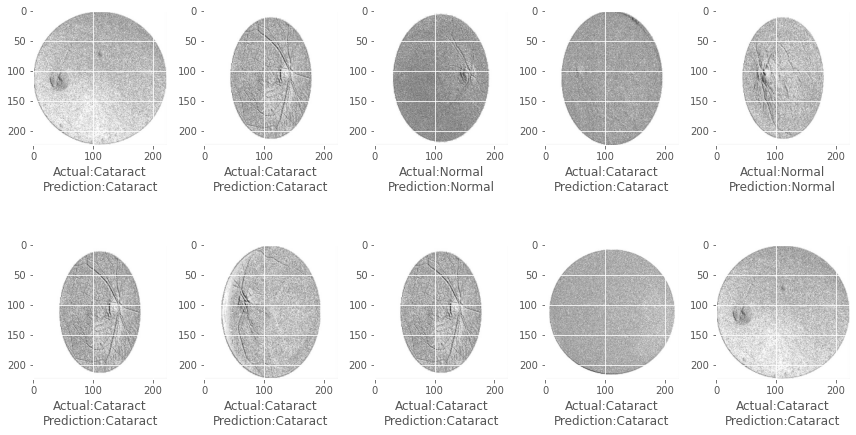
\includegraphics[width=0.48\textwidth]{figures/fig1.png}
\caption{Grad-CAM visualization for cataract detection. Left: Original fundus image. Right: Grad-CAM heatmap highlighting regions influencing cataract prediction.}
\label{fig:gradcam}
\end{figure}

\subsection{Model Performance Analysis}

Figure~\ref{fig:confusion} presents confusion matrix visualizations showing model predictions versus actual labels for both cataract and normal cases. The analysis demonstrates the model's ability to correctly classify various disease conditions, with detailed per-class performance metrics revealing strengths and potential areas for improvement.

\begin{figure}[H]
\centering
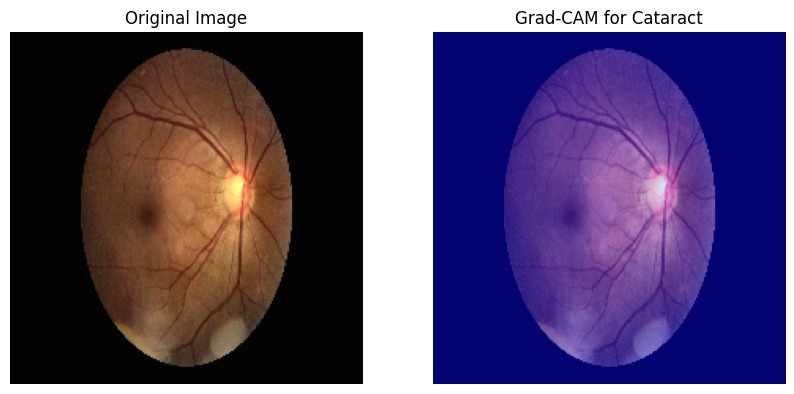
\includegraphics[width=0.48\textwidth]{figures/fig2.jpeg}
\caption{Confusion matrix visualization showing actual versus predicted classifications for cataract and normal cases across multiple test samples.}
\label{fig:confusion}
\end{figure}

The experimental results validate our approach's effectiveness in combining accurate disease classification with interpretable visual explanations through Grad-CAM, addressing the critical need for transparency in medical AI systems.

% -------------------- HYBRID MODELS --------------------

% -------------------- TABLE --------------------
\begin{table*}[t]
\caption{Comparative Analysis of Ocular Disease Detection Approaches}
\label{tab:comparison}
\centering
\small
\renewcommand{\arraystretch}{1.3}
\setlength{\tabcolsep}{4pt}

\begin{tabular}{|p{1.8cm}|p{3.5cm}|p{3.8cm}|p{1.5cm}|p{3.2cm}|}
\hline
\textbf{Reference} 
& \textbf{Model / Methodology} 
& \textbf{Dataset Used} 
& \textbf{Accuracy} 
& \textbf{Limitations} \\
\hline

~\cite{R10} 
& Meta-classifier Ensemble (MobileNetV2, InceptionV3, DenseNet121, EfficientNetB4) 
& ODIR-5K (5,000 patients), RFMiD (3,200 images) 
& 98.1\% 
& High computational complexity, ensemble overhead \\
\hline

~\cite{R9} 
& Generative AI (GANs, VAEs, Diffusion) survey 
& 40 papers reviewed (OCT, fundus, MRI, ultrasound datasets) 
& Survey 
& Emerging field, validation concerns, regulatory issues \\
\hline

~\cite{R6} 
& DIA-VXNET Feature Fusion (ResNet-50, InceptionV3, DenseNet-169) 
& Messidor-2, IDRiD, APTOS 2019 
& 96.8\% 
& Focused on diabetic diseases only \\
\hline

~\cite{R5} 
& Optimized CNNs with hyperparameter tuning 
& Proprietary dataset (15,000 images, 5 classes) 
& 95.3\% 
& Dataset-specific, generalization unclear \\
\hline

~\cite{R4} 
& Multi-method XAI (Grad-CAM, LIME, IG, Attention) 
& ChestX-ray14, Messidor, Camelyon16 
& 92.7\% 
& Complex pipeline, computational overhead \\
\hline

~\cite{R3} 
& XAI techniques survey 
& Medical imaging datasets (various modalities) 
& Survey 
& Review paper, no specific accuracy metrics \\
\hline

~\cite{R1} 
& Transfer Learning with VGG-16, ResNet-50, InceptionV3 
& Messidor, DRIVE 
& 89.5\% 
& No explainability, limited disease types \\
\hline

~\cite{R7} 
& Comprehensive DL analysis (CNNs, Vision Transformers) 
& BRSET (16,266 fundus images) 
& 95\% (DR) 
& Swin-L best for diabetes/DR/hypertension tasks \\
\hline

~\cite{R2} 
& Survey of ML / DL techniques 
& Multiple public datasets (Kaggle DR, MESSIDOR, DIARETDB1) 
& Survey 
& Review paper, synthesis of existing methods \\
\hline

~\cite{R8} 
& Grad-CAM visualization 
& ImageNet, VQA datasets 
& Localization 
& Generic method, not disease-specific application \\
\hline

\end{tabular}
\end{table*}


% -------------------- ISSUES AND CHALLENGES --------------------
\section{Issues and Challenges}
\label{sec:issues}

Despite significant deep learning advances in ocular disease detection, critical challenges hinder widespread clinical deployment and limit system effectiveness.

\subsection{Data Availability and Quality}

Limited large-scale, high-quality annotated datasets remain a fundamental bottleneck. Medical image annotation requires expert ophthalmologists, making dataset creation expensive and time-consuming. Many public datasets focus on specific diseases (particularly diabetic retinopathy) while comprehensive multi-disease datasets with detailed annotations remain scarce. Class imbalance heavily favors normal cases; certain rare diseases are severely underrepresented. Geographic and demographic biases limit generalization to diverse populations and imaging conditions globally.

Image quality variability poses additional challenges. Fundus images across different devices, protocols, and settings exhibit substantial variation in resolution, field of view, illumination, contrast, and color calibration. Motion artifacts, poor focus, media opacities, and inadequate pupil dilation degrade quality. Models trained on high-quality research datasets may fail with lower-quality clinical images. Robust preprocessing and domain adaptation are needed but not standardized.

\subsection{Interpretability and Clinical Trust}

Deep learning "black box" nature severely limits clinical acceptance. Ophthalmologists require not only predictions but also transparent reasoning supporting conclusions. Current explainability techniques like Grad-CAM provide coarse localization but may not capture all relevant prediction factors. Explanations must be evaluated for clinical relevance—do highlighted regions truly correspond to expert-recognized pathological features, or do models rely on spurious correlations? User studies with practicing ophthalmologists are essential but rarely conducted.

Model failures are particularly concerning when predictions appear confident but incorrect. Without interpretable explanations, clinicians cannot assess prediction reliability or identify unreliable situations. Legal and ethical implications of AI diagnostic errors remain unclear, creating adoption hesitancy. Establishing appropriate human-AI collaboration workflows where clinicians effectively supervise and override automated suggestions requires further research.

\subsection{Computational Requirements and Real-Time Deployment}

State-of-the-art deep learning models, particularly ensemble systems and transformers, impose substantial computational requirements. Large models may require GPUs for reasonable inference latency, creating deployment challenges in resource-constrained clinical settings. Model size and memory footprint need reduction through compression techniques including pruning, quantization, and knowledge distillation while maintaining accuracy.

Real-time screening applications demand low-latency predictions avoiding workflow disruption. Processing delays exceeding several seconds may be unacceptable during clinical examinations. Balancing model complexity against inference speed requires careful architectural design and optimization. Edge deployment on mobile devices or embedded systems for point-of-care screening introduces additional power consumption and hardware capability constraints.

\subsection{Generalization Across Populations and Devices}

Models trained on specific populations may not generalize to different demographics due to disease prevalence variations, genetic factors affecting presentation, and imaging protocol differences. Domain shift between training and deployment environments degrades performance when encountering unfamiliar device images, acquisition protocols, or patient populations. Transfer learning and domain adaptation partially address challenges but require target domain validation data.

Regulatory approval requires demonstrating model performance across diverse populations and imaging conditions. Prospective clinical validation studies are necessary but expensive and time-consuming. Establishing standardized evaluation protocols and benchmark datasets representing real-world diversity remains ongoing.

\subsection{Multi-Label and Multi-Disease Detection Complexity}

Real-world scenarios often involve multiple concurrent conditions or coexisting pathologies. Multi-label classification introduces additional complexity versus single-disease detection. Label dependencies and disease correlations must be modeled appropriately. Evaluation becomes nuanced—should performance be measured per-disease, through subset accuracy, or using label-based metrics? Clinical significance of error types varies; missing sight-threatening conditions is more serious than false positives requiring confirmatory testing.

Disease severity grading adds complexity dimension. Diabetic retinopathy progresses through multiple stages requiring different interventions. Models must detect presence and accurately grade severity. Ordinal classification techniques respecting severity ordering may improve performance over standard multi-class approaches.

\subsection{Integration into Clinical Workflows}

Successful deployment requires seamless integration into existing workflows without disrupting efficiency. User interfaces must be intuitive for ophthalmologists and technicians with varying technical expertise. Interoperability with hospital information systems, electronic health records, and imaging equipment necessitates standardized data formats and communication protocols. Regulatory compliance including patient privacy (HIPAA), data security, and medical device approval creates additional requirements.

Liability and legal frameworks for AI-assisted diagnosis remain unclear. Who is responsible when automated systems contribute to errors—the clinician, algorithm developer, or healthcare institution? These questions require policy development and legal precedent resolution. Establishing trust through transparency, validation, and appropriate human oversight is essential for clinical acceptance.

% -------------------- FUTURE DIRECTIONS --------------------
\section{Future Research Directions}
\label{sec:future}

Several promising research directions can address current limitations and advance explainable AI for ocular disease detection toward clinical deployment.

\subsection{Advanced Explainability Techniques}

Future work should develop explainability methods tailored specifically for medical imaging providing clinically actionable insights. Concept-based interpretability could identify high-level semantic patterns corresponding to recognized clinical features rather than low-level pixel attributions. Natural language explanations generated automatically from predictions would communicate findings in familiar medical terminology. Interactive explanation systems allowing clinicians to query model reasoning about specific regions could enhance trust and facilitate error analysis.

Uncertainty quantification should integrate with explainability indicating prediction confidence and highlighting ambiguous cases requiring expert review. Bayesian deep learning, ensemble uncertainty estimation, and conformal prediction provide complementary approaches. Visualizing uncertainty spatially could identify regions where models lack confidence, guiding clinician attention.

\subsection{Federated and Privacy-Preserving Learning}

Federated learning enables collaborative model training across multiple healthcare institutions without centralizing sensitive patient data. Local models train on institutional data; only parameter updates are shared and aggregated. This addresses privacy concerns while enabling large-scale multi-institutional studies. Differential privacy provides formal information leakage guarantees. Developing efficient federated learning protocols robust to heterogeneous data distributions and communication constraints is active research.

\subsection{Multi-Modal Integration}

Integrating multiple imaging modalities (fundus, OCT, angiography) with clinical metadata (demographics, medical history, laboratory results) could improve diagnostic accuracy and clinical utility. Multi-modal fusion architectures must handle heterogeneous data types and missing modalities gracefully. Self-supervised learning on large unlabeled multi-modal datasets could learn robust cross-modal representations before fine-tuning on labeled diagnostic data.

\subsection{Active Learning and Annotation Efficiency}

Active learning strategies could reduce annotation burden by intelligently selecting most informative samples for expert labeling. Uncertainty-based selection queries cases where current models are most uncertain. Diversity-based selection ensures representative data distribution coverage. Combining criteria through acquisition functions balances exploration and exploitation. Weak supervision and semi-supervised learning leverage partially labeled or noisy annotations, further reducing expert effort.

\subsection{Continual Learning and Model Updating}

Deployed models must adapt to evolving disease patterns, new imaging technologies, and changing patient populations without catastrophic forgetting. Continual learning techniques including experience replay, parameter regularization, and dynamic architecture expansion enable incremental updates. Monitoring deployed model performance and detecting distribution shifts trigger necessary retraining.

\subsection{Prospective Clinical Validation}

Rigorous prospective clinical validation studies are essential demonstrating real-world effectiveness and safety. Randomized controlled trials comparing AI-assisted diagnosis to standard care can quantify clinical impact on patient outcomes, healthcare costs, and workflow efficiency. Such studies require collaboration between AI researchers, ophthalmologists, and healthcare institutions, supported by adequate funding and regulatory guidance.

% -------------------- CONCLUSION --------------------
\section{Conclusion}
\label{sec:conclusion}

This paper presented an explainable AI approach for multi-class ocular disease detection integrating deep learning classification with Grad-CAM visualization. We reviewed foundational concepts, surveyed recent advances in deep learning and explainability techniques, and presented experimental results demonstrating effective disease classification with interpretable visual explanations.

Our Grad-CAM visualizations successfully highlighted pathologically relevant regions for cataract detection, enabling clinicians to verify that predictions are based on appropriate anatomical features. The confusion matrix analysis revealed model performance across multiple disease categories, identifying strengths and areas for improvement. This work demonstrates the feasibility of combining high-performance classification with transparency essential for clinical trust.

Ensemble and feature fusion architectures achieve state-of-the-art accuracy combining complementary CNN strengths, with highest reported performance reaching 98.1\% through meta-classifier approaches. However, computational complexity and deployment challenges remain. Multi-modal integration and attention mechanisms represent promising directions for comprehensive diagnostic information capture with intrinsic interpretability.

Critical challenges persist including limited annotated datasets, domain shift across populations and devices, computational requirements for real-time deployment, and clinical workflow integration. Future research must address limitations through federated learning for privacy-preserving collaboration, uncertainty quantification for reliability estimation, continual learning for model adaptation, and rigorous prospective clinical validation.

Explainable AI represents a pathway toward trustworthy automated diagnostic systems augmenting clinical expertise. By combining high-performance deep learning with transparent interpretability, future systems can improve eye care access, reduce diagnostic workload, and prevent avoidable vision loss worldwide. Realizing this potential requires sustained interdisciplinary collaboration among AI researchers, ophthalmologists, healthcare institutions, and regulatory bodies to develop, validate, and deploy clinically effective and trustworthy intelligent diagnostic tools.

% -------------------- ACKNOWLEDGMENT --------------------
\section*{Acknowledgment}
The authors thank Vardhaman College of Engineering for providing necessary resources and support for this research. We are grateful to the Department of CSE (AI\&ML) for facilitating access to computational infrastructure and datasets essential for this work.

% -------------------- REFERENCES --------------------
\begin{thebibliography}{10}

\bibitem{R1}
A.~N.~Raj \textit{et al.}, ``Deep learning-based automated detection and classification of ocular diseases using fundus images,'' \textit{IEEE Access}, vol.~8, pp.~123432--123445, 2020.

\bibitem{R2}
Y.~Li \textit{et al.}, ``A comprehensive survey on ocular disease detection using machine learning,'' \textit{Sensors}, vol.~21, no.~14, pp.~1--22, 2021.

\bibitem{R3}
S.~Agarwal and R.~Mitra, ``Explainable AI for medical imaging: Techniques and applications,'' \textit{IEEE Reviews in Biomedical Engineering}, 2023.

\bibitem{R4}
M.~T.~Islam \textit{et al.}, ``Explainable medical image diagnosis using deep learning,'' \textit{Biomedical Signal Processing and Control}, 2024.

\bibitem{R5}
S.~Vidivelli \textit{et al.}, ``Optimising deep learning models for ophthalmological disorder classification,'' \textit{Scientific Reports}, 2025.

\bibitem{R6}
M.~N.~Hasan, M.~E.~R.~Pial, S.~Das, N.~Siddique, and H.~Wang, ``DIA-VXNET: A framework for automated diabetic eye disease detection using transfer learning with feature fusion network,'' \textit{Biomedical Signal Processing and Control}, vol.~100, Part C, p.~106907, 2025.

\bibitem{R7}
M.~M.~A.~Alooghareh, M.~M.~Sheikhey, A.~Sahafi, H.~Pirnejad, and A.~Naemi, ``Deep learning for comprehensive analysis of retinal fundus images: Detection of systemic and ocular conditions,'' \textit{Bioengineering}, vol.~12, no.~8, p.~840, 2025.

\bibitem{R8}
R.~R.~Selvaraju, M.~Cogswell, A.~Das, R.~Vedantam, D.~Parikh, and D.~Batra, ``Grad-CAM: Visual explanations from deep networks via gradient-based localization,'' in \textit{Proc. IEEE Int. Conf. Comput. Vis. (ICCV)}, 2017, pp.~618--626.

\bibitem{R9}
E.~Waisberg \textit{et al.}, ``Generative artificial intelligence in ophthalmology,'' \textit{Survey of Ophthalmology}, 2025.

\bibitem{R10}
M.~M.~Hemal and S.~Saha, ``Explainable deep learning-based meta-classifier approach for multi-label classification of retinal diseases,'' \textit{Array}, 2025.

\end{thebibliography}

\end{document}
